\textbf{PROBLEMA 2}
\vspace{20px}

\newcommand{\ivec}{\boldsymbol{\hat{\imath}}}
\newcommand{\jvec}{\boldsymbol{\hat{\jmath}}}
\newcommand{\kvec}{\boldsymbol{\hat{k}}}

Tres alambres infinitos paralelos entre sı́ y perpendiculares al plano de la hoja se ubican en los vértices de
un cuadrado de lado $d$. Uno de ellos lleva corriente $2I$ que entra al plano, mientras que los otros llevan corriente
$I$ que emerge del plano de la hoja.\\

\begin{enumerate}[label=\alph*.]
    \item Calcule el vector campo magnético en el punto $P_1$.
    \item Calcule la fuerza que actúa sobre una carga $q$ con velocidad $\mathbf{v} = 3 \ivec
    + 2 \jvec  + \kvec$̃ situada en $P_1$.
    \item Supongamos que se traslada una carga desde el punto $P_1$ al punto $P_2$ a lo largo de la lı́nea recta que une
    esos dos puntos, ¿cuál es el trabajo que cuesta dicho traslado?
\end{enumerate}

\begin{center}
    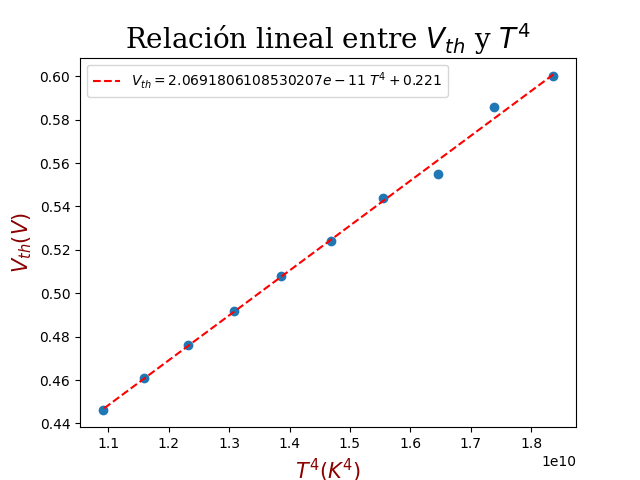
\includegraphics[width=10cm]{files/img2}
\end{center}

\vspace{20px}
\textit{Solución:}
\\

\textbf{a}. De acuerdo al principio de superposición, el campo magnético en el punto $P_1$ será la suma del campo magnético generado
por cada uno de los alambres. Podríamos calcular la contribución de cada alambre mediante la ley de Biot y Savart,
pero considerando la simetría del problema, y que los alambres son infinitos, es más fácil obtener la solución a partir de la ley
de Ampère.\\

\begin{equation*}
    \[ \oint_C \vec{B} \cdot d\vec{\ell} = \mu_{0}I_C \]
\end{equation*}


El campo magnético es constante a la largo de una curva circular por cuyo centro pasa el alambre, y su dirección es tangente a esta
circunferencia. Su módulo es $B = \frac{\mu_{0}I_C }{2\pi R}$. En la siguiente figura se representan los 3 campos magnéticos con sus
direcciones respectivas.


\begin{center}
    \begin{tikzpicture}
%    \draw[thin,gray!40] (-2,-2) grid (2,2);
        \draw[<->] (-2.5,0)--(2.5,0) node[right]{$x$};
        \draw[<->] (0,-2.5)--(0,2.5) node[above]{$y$};

        \draw[dashed] (-2,2)--(2,2) node[above,xshift=-2.4cm] {$d$};
        \draw[dashed] (-2,2)--(-2,-2) node[left,yshift=2.4cm] {$d$};;
        \draw[dashed] (-2,-2)--(2,2);



        \draw (-2,2) circle (6pt) node[above left=6pt]{$\boldsymbol{1}$};
        \draw (-2,2) pic[rotate = 0] {cross=4pt};

        \draw (2,2) circle (6pt) node[above right=6pt]{$\boldsymbol{2}$};
        \filldraw (2,2) circle (3pt);

        \draw (-2,-2) circle (6pt) node[below left=6pt]{$\boldsymbol{3}$};
        \filldraw (-2,-2) circle (3pt);


        \draw[line width=2pt,red,-stealth](0,0)--(-1,-1) node[anchor=east]{$\boldsymbol{\vec{B_1}}$};
        \draw[line width=2pt,blue,-stealth](0,0)--(0.5,-0.5) node[anchor=west]{$\boldsymbol{\vec{B_2}}$};
        \draw[line width=2pt,blue,-stealth](0,0)--(-0.5,0.5) node[anchor=south]{$\boldsymbol{\vec{B_3}}$};
    \end{tikzpicture}
\end{center}

La distancia de cada alambre al punto $P_1$ es $d / \sqrt{2}$. Observamos que los campos $\boldsymbol{\vec{B_}}_2$ y $\boldsymbol{\vec{B}}_3$ se cancelan por tener direcciones opuestas
y mismo módulo, por lo que el campo en el punto $P_1$ es $\boldsymbol{\vec{B}}_1$ .


\begin{equation*}
    \boldsymbol{\vec{B}}_{P1} = \boldsymbol{\vec{B}}_1 = \frac{\mu_{0} 2 I \sqrt{2} }{2 \pi d} \left( -\cos(45\degree )\ivec -\sen(45\degree)\jvec \right)
    = \frac{\mu_{0} I}{\pi d} \left( -\ivec -\jvec \right)
\end{equation*}


\textbf{b}. La fuerza de Lorentz describe la fuerza que actúa sobre una carga puntual en movimiento en presencia de un campo magnético.

\begin{equation*}
    \boldsymbol{\vec{F}} = q \boldsymbol{\vec{v}} \times \boldsymbol{\vec{B}}
\end{equation*}

Conocemos tanto $\boldsymbol{\vec{v}}$ como $\boldsymbol{\vec{B}}$, por lo que podemos realizar el producto vectorial para calcular la fuerza
que actúa sobre la carga $q$.

\begin{equation*}
    \boldsymbol{\vec{F}} = q \; \frac{\mu_{0} I}{\pi d} \left[(3 \ivec
    + 2 \jvec  + \kvec)  \times \left( -\ivec -\jvec \right)  \right] =
    \frac{\mu_{0} q I}{\pi d} (\ivec - \jvec - \kvec )
\end{equation*}

\textbf{c}. La fuerza magnética que actúa sobre una partícula cargada que se mueve a través de un campo magnético es siempre perpendicular a la
velocidad de la partícula. La fuerza magnética modifica la dirección de la velocidad, pero no su módulo. Por lo tanto,
los campos magnéticos no realizan trabajo sobre las partículas y no modifican su energía cinética. El trabajo que cuesta el traslado
de una carga desde el punto $P_1$ al punto $P_2$ es nulo.